\chapter{Background and Related work}
In this chapter, we will introduce context on which our work is based. For full overview, we must familiarize the reader with the following concepts: Big Data, NoSQL, MapReduce, YARN, Spark, JSON, JSONiq and finally Rumble.

Test Driver itself will be built as a layer on top of Rumble. Because of the architecture which enables data independence, we do not need to know its underlying structure. However, seeing the full architecture and having an overview will help us make decisions throughout this work.

\section{Big Data}
Big Data in today's world has a broad scope and several definitions. Here we will present a certain view of the Big Data on which Rumble was based. We can look at the data being "big" in the following 3 dimensions \cite{BigDataCourse}:%from 01 Big Data - Introduction although I updated from 2020 lecture}:
\begin{itemize}
	\item Volume - This term simply corresponds to the number of bytes that our data consists of. To have an idea of the scale, in Big Data, we are often looking at PBs of data. Scientific centers such as CERN produce tens of PBs of data annually. The information, the data in today's world brings value. Not only scientific centers, but also big companies gather data, store it in their data centers and process it in order to extract this value.
	\item Variety - Data often comes in different shapes. The most familiar ones are text - completely unstructured data, followed by data organized as cubes, tables, graphs, or trees on which we will mainly focus. Until 2000's, the world was mainly oriented towards relational databases for which the underlying shape is a table. The main focus was on introducing normalization forms with the idea to avoid data redundancy. Then the tables would simply be joined using SQL as the query language via the foreign keys. However, starting from 2000's relational databases and SQL could not satisfy the needs of real-world scenarios. Often data is unstructured, nested, values are missing, etc. This trend led to Not Only SQL - NoSQL databases. The main focus in NoSQL database is to perform opposite and actually de-normalize the data. Looking at the table, we would now allow non-atomic values in a single cell or even missing values. Such a transition leads the data shape to transform from flat homogeneous tables to nested heterogeneous trees. Choosing the correct data shape is essential. What CSV and SQL were in a relational database, for tree-shaped data we have JSON and XML as a data format with JSONiq and XQuery as their respective querying languages.
	\item Velocity - Data, in the end, is physically stored on some medium drive. The 3 main factors of this underlying medium drive are capacity, throughput and latency. From mid 1950's until today, we have witnessed a tremendous increase in all 3 factors. Capacity has increased by up to 200 x $10^9$, throughput by 10 x $10^3$  and latency by 8 times. This ever-growing discrepancy between factors has brought needs for parallelization and batch processing. Since a single medium drive has increased capacity much more than throughput, we need to read data from multiple medium drives simultaneously in parallel to obtain data fast enough. At the same time, to face the discrepancy between throughput and latency, we need to obtain data in batches. Thus, the need for systems that can perform parallel batch processing has increased.
\end{itemize}
In summary, traditional Relational Database Management System - RDBMS, such as Oracle database or Microsoft SQL Server, have focused on being compliant with ACID (atomicity, consistency, isolation and durability) properties. Such RDBMSes with homogeneous tables are good when handling a small amount of data. However, if we need to scale the data massively, we need to turn to different technologies. These traditional RDBMSes that use file systems such as FAT32 or NTFS for physical storage are not sufficient \cite{BigDataCourse}. %from 02 Big Data - Lessons learn

On the other hand, NoSQL databases are compliant with the CAP (consistency, availability, partition tolerance) theorem.  Examples of new NoSQL databases that have emerged are key-value stores (DynamoDB), document stores (MongoDb) and column-oriented stores (HBase). They often use Distributed File System (DFS) as physical storage such as HDFS. Instead of traditional scaling up, by buying single high-performance hardware, the orientation is towards scaling out by buying a lot of cheap commodity hardware. Such scaling enables that hardware costs grow linearly with the amount of data.  These concepts lead to building high-performance and scale-able frameworks such as Hadoop that can query and process distributed massive quantities of data in parallel \cite{BigDataCourse}. %rom 03 Data in the Large - Object and Key-Value Storage

\section{Hadoop}
Apache Hadoop \cite{Hadoop} is an open-source framework written in Java that is able to manage big data, store it and process it in parallel in a distributed way across a cluster of commodity hardware. It consists of 3 components \cite{BigDataCourse}: %from 04 Data in the Large - Distributed File systems and Exercise03 HDFS
\begin{itemize}
	\item HDFS - Storage layer
	\item MapReduce - Processing layer
	\item YARN - Resource management layer
\end{itemize}

In this section, we will briefly introduce each of the layers. It will help the reader to better understand Spark in the upcoming chapter.

\subsection{HDFS}
The Hadoop Distributed File System - HDFS \cite{HDFS} is a physical storage layer of Hadoop inspired by Google File System - GFS \cite{GFS} written in Java. It is one of the most reliable file systems for storing big data distributed on a cluster of commodity hardware. In this section, we need to understand how HDFS physically stores big data on the machines. When we say big data, we are thinking at the scale of millions of PB files. This means that files are bigger than a single drive (medium). Therefore, in such a setting, the most suitable is block storage. Unlike a typical NTFS system with allocation units of 4 KB, the block size is by default 64 or 128 MB. It is chosen as a good trade-off between latency and replication. Transferring multiple blocks bigger than 4 KB will reduce latency and also reduce the network overhead. When it comes to replicas, each block has by default 3 copies in case of a failure.  

The architecture is master-slave. Master is NameNode and it is in charge of storing a namespace. The namespace is a hierarchy of files and directories. Since the blocks are 64 or 128 MB, the metadata is also small. And since we are storing a rather small amount of very large files, the whole namespace can fit in the RAM of the NameNode. In addition to the namespace, NameNode knows the file to blocks mapping together with the location of blocks and its replicas. The blocks are stored on DataNodes that act as slaves. When clients want to read/write the files, they communicate with NameNode only once to receive the locations meaning that NameNode is not the bottleneck. 

Such an architecture allows potential infinite scalability just by adding DataNodes, meaning that hardware cost grows linearly with the increase of data. The single point of failure is NameNode, meaning that we have consistency and partition tolerance at the cost of availability from CAP theorem. In case of a failure, there is a secondary NameNode that would start-up. Also, it enables high durability with 3 replicas and read/write performance. When reading, it usually transfers a lot of data - batch processing.

\subsection{MapReduce}
MapReduce \cite{MapReduce} in its most broad definition is a programming model (style) answering the question of how we process the data. It consists of two crucial steps map and reduce alongside with shuffle as the intermediate step \cite{BigDataCourse}: %from 06 Data in the Large - Massive Parallel Processing
\begin{itemize}
	\item Map - Input data is mapped into an intermediate set of key-value pairs
	\item Shuffle - All key-value pairs are shuffled in a way such that all pairs with the same key end up same machine
	\item Reduce - Data is aggregated on the machine and the output is produced
\end{itemize}
Example - Count occurrences of each word in a document of 1000 Pages:

\begin{enumerate}
	\item What we can do is that we can first have a single map task per page. This way, those 1000 pages can be done in parallel. The map task will perform Map (K1, V1) $->$ List (K2, V2), where K1 is in the range from 1 to 1000 (for each page) and V1 is the text on each page. K2 will have values in the range of all possible words that occur in the document. V2 will always be 1. Such a mapper is very primitive. If reduce task is a commutative and associative function, then it is allowed to execute the same function in the map task to reduce the amount of shuffle that will happen afterward. As count is such a function, we can already perform sum per key in the map task. It means that K2 stays the same and V2 will be the actual count per page.
	\item As not all possible words will appear on all pages, we will simply put together a collection of all the produced key-value pairs and sort them per key. We will then assign all key-value pairs with the same key to the single reducer and partition the data accordingly.
	\item Reduce task will perform (K2, List (V2)) $->$ List (K2, V3) - reducer can output the same key-value pair, but in general it can be any other. Finally, V3 will be the sum of occurrences of the word K2.
\end{enumerate}
   
In general, MapReduce as a programming model can be used in any framework with any underlying physical storage such as local file system, S3, Azure, HDFS. Here we will describe infrastructure in Hadoop Version 1 where it is running on top of HDFS where we also have Resource Management layer. It is again master-slave architecture where we have JobTracker and TaskTracker. JobTracker is the master with responsibilities of Resource Management, Scheduling, Monitoring, Job lifecycle and Fault-tolerance. One job consists of multiple tasks, depending on how the data is split. And 1 task can be a map or reduce task. One or more tasks are then assigned to TaskTracker that needs to execute them. JobTracker is collocated with NameNode and TaskTracker, usually with the DataNode, in order to bring query to the data. 

\subsection{YARN}
Yet Another Resource Negotiator -  YARN \cite{YARN} is a Resource Management layer in Hadoop Version 2. Comparing to Version 1, we might notice that JobTracker has many responsibilities. It is responsible for both types of jobs, scheduling and monitoring ones. JobTracker is acting as the "Jack of all trades" and becoming a bottleneck in such a setting. Such bottleneck leads to scale-ability issues and Hadoop could not handle more than 4000 nodes executing more than 40000 tasks (remember that job comprises a set of task). 

The solution was introducing YARN that separates scheduling and monitoring responsibilities. The architecture is again master-slave where we have ResourceManager and NodeManager. It has a single ResourceManager per cluster in charge of only scheduling and performs: capacity guarantees, fairness, SLA, cluster Utilization, assigns containers. It has a global overview of all cluster resources and provides leases for containers. One node in a cluster has one NodeManager and many containers. A container is an abstraction in which task can be run and it comprises a set of resources such as RAM, CPU, Storage, Bandwidth that can be allocated to ApplicationMaster. ApplicationMaster has the responsibility to handle monitoring. In particular, it is in charge of: fault tolerance, monitoring, asking for resources, tracing job progress/status, heart-beating to the ResourceManagerr, Ability to handle multiple jobs. We have many ApplicationMasters in a cluster, each job has one ApplicationMaster, but not every node has to have an ApplicationMaster. In essence, it can happen that a single node has multiple ApplicationMasters, each responsible for a different job completely unaware of the existence of other ApplicationMasters on the node. Finally, it should be noted that ApplicationMaster is a container. Described architecture solves the bottleneck issue allowing the cluster to scale up to 10000 nodes and 100000 tasks \cite{BigDataCourse}. %from 07 Data in the Large - Resource Management and Exercise 06 Spark

Full flow of duties overview:
\begin{itemize}
	\item Clients submits a job. 
	\item ResourceManager creates a job and returns ID. \item Client sends its requirements. 
	\item ResourceManager tells a NodeManager to promote one of containers to ApplicationMaster. 
	\item ResourceManager tells maximum capacity of containers. 
	\item ApplicationMaster requests containers. 
	\item ResourceManager assigns containers.
\end{itemize}


YARN offers a couple of types of schedulers, that based on application and its request in terms of resources, perform the allocation.

\section{Spark}
Apache Spark \cite{ApacheSpark} \cite{SparkDefinitiveGuide} \cite{LearningSpark} is is an open-source engine for large-scale data processing. We see it as a generalization of MapReduce. From a straight pipeline of two tasks, map and reduce, it generalizes it to any Directed Acyclic Graph - DAG. DAGs are built around Resilient Distributed Datasets - RDDs \cite{RDD} which are an abstraction for partitioned collection of values. On RDDs, we can perform creation, transformation and action. In Spark we need to make a clear separation of two plans, two graphs - lineage and DAG.

DAG is a physical plan of execution. A DAG is created when the user creates an RDD (by referencing a dataset in an external file system for example) and applies chains of lazy transformations on it. When action is called, it triggers the computation. The DAG is given to the DAG Scheduler, which divides it into stages of tasks. A stage is comprised of tasks based on partitions of the input data. The stages are passed on to YARN that now executes them physically. Since Spark has end-to-end DAG, it can figure out which tasks can be done in parallel. All these will then run into parallel on several nodes \cite{BigDataCourse}. %from 08 Data in the Large - Massive Parallel Processing (SPARK) and Exercise 06 Spark)

Lineage graph tells us a logical plan. It tells us which RDD originates from which RDD. All the dependencies between the RDDs will be logged in the lineage graph rather than the actual data. This is called lazy evaluation, it only gets triggered when action is called. This lineage is used to recompute the RDD in case of failure.

Fault tolerance using lineage - Imagine that we start with an RDD on which we need to perform a couple of transformations and finally an action. Such RDD would first get partitioned so that multiple nodes can handle it. Imagine that some node fails, it means that only the partitions located on that node have to be recomputed. And the lineage graph is telling us exactly which set of transformations is needed to reconstruct the RDD.

DataFrame is a high-level abstraction of RDD's. It is a logical data model that enables users to view and manipulate data independently of physical storage. DataFrames store data in a collection of rows enabling the user to look at RDD's as tables. They are nothing more than named columns like we had before. Therefore, we can use high-level declarative language - Spark SQL to query the data without caring about underlying physical storage.

The main problem with DataFrames is that heterogeneous data that we are encountering in tree data shapes cannot fit in DataFrame. The de-normalization that enabled nested, missing values or values of a different type will not work. Running Spark on such dataset results in Spark skipping and leaving to the user to manually handle heterogeneous data. DataFrames are simply not the correct representation for the tree-shaped data. 

\subsection{Apache Spark vs .Apache Hadoop MapReduce}
For emphasizing the power of Spark, we have found a nice comparison with Hadoop MapReduce that can be separated into the following categories: 
\begin{itemize}
	\item Performance - Hadoop MapReduce stores the output on the disk after each map or reduce task. Spark keeps everything in memory. Spark performs better if all data is stored in RAM. If RAM is full, Spark uses disk, but overall it is better.
	\item Ease of use - Spark has compatible API for Python, Scala, Java. On the other hand, Hadoop MapReduce is written in Java, and it is hard to learn the syntax for programming. 
	\item Cost - Spark needs a lot of RAM, so it is more expensive. All data needed for a job has to fit in RAM
	\item Data processing - Spark can do graph, ML, batch, and real-time processing, making it one platform for everything. Hadoop MapReduce is good for batch processing, but it does not support graph or real-time processing. 
	\item Fault tolerance - Hadoop MapReduce relies on hard drives. In case of failure, it can continue wherever it left off and save time. It also has replication for fault tolerance. Spark uses RDDs for fault tolerance. They can refer to any dataset in external storage like HDFS. If RDD is lost, it is recomputed using transformations.
\end{itemize}

\section{Querying Language}
\subsection{JSON}
\label{sec:JSON}
JavaScript Object Notation - JSON \cite{JSON}is a text-only, human-readable data format. It originates from JavaScript, but today it is a widely spread language-independent data format supported by many programming languages. 

As we have seen, DataFrames in Spark and table data shape in general, which can be stored in CSV data format, is not suitable for heterogeneous data and de-normalization does not work. On the other hand, tree data shape and JSON as the data format is the perfect choice for nested heterogeneous data. It supports nesting by using 2 structured data types:
\begin{itemize}
	\item Object - a collection of key-value pairs that act as an associative array (map) from string to any other type 
	\item Arrays - ordered sequence of items of any type. 
\end{itemize} 

JSON also supports the four atomic data types that can be String, Number, Boolean and Null.

To better understand why JSON is good for nested data, we will provide an example. The code below shows that the value of the address is a nested JSON object consisting of two more nested JSON objects. Also, skills that have multiple values are presented using a JSON array.

\lstinputlisting[language=json]{json_example.json}

\subsection{JSONiq}
\label{sec:JSONiq}
JSONiq \cite{JSONiqPaper}, as mentioned in the introduction, is a declarative and functional querying language created exactly to analyze files written in JSON data format. It is designed to analyze tree-shaped data - nested and heterogeneous. It inherits 95\% of its features from XQuery, its XML counterpart. It has a data model that can capture all aspects of JSON data format. 

We say it is declarative because the user does not need to be aware of the underlying structure. It is a query language like SQL in the RDBMS, with the difference that it operates on JSON.

When it comes to the data model, everything is expressed as a Sequence of Items. Item itself can be any of the 6 data types that JSON supports. In addition, Ian Item can also be a Function. Then all Expressions that exist operate only on Sequence of Items. 

We say it is functional because Expression takes Sequence of Items as the input and produces again Sequence of Items as the output. It means that Expressions can be nested in any desired way.

The Expressions can be organized in the following categories:
\begin{multicols}{2}
	\begin{itemize}
		\item Arithmetic
		\item Logic
		\item Comparison
		\item Literal
		\item JSON construction
		\item JSON navigation
		\item Sequence Construction
		\item Built-in function
		\item FLWOR expression
		\item Variable references
		\item Context item references
		\item Named function references
		\item Control flow expressions
		\item Type 
		\item Static function calls
		\item Dynamic function calls
	\end{itemize}
\end{multicols}

FLWOR expression is the most powerful. Using its own clauses, it is capable of everything Select From Where in SQL does - Selection, Projection, Grouping, Ordering, Join. It can also be nested any number of times in almost any order which SQL does not quite support \cite{JSONiqBook}. To fully understand the power of FLWOR expression, we will provide an example. It is pretty declarative and intuitive for everyone who had a chance to write an SQL query before. We first select persons living in Glattbrugg. Then we are grouping them by nationality. Finally, we count persons in groups and select only those with more than 1000 to be displayed ordered. We can see freedom in writing this query - where can be applied multiple times, also let can be placed anywhere.

%in,
\lstinputlisting[language=XML, frame=single, breaklines=true, showspaces=false,,otherkeywords={descending, for, where, eq, group, let, where, gt, order, by, return}, stringstyle=\color{ao}, keywordstyle=\color{chromeyellow}]{jsoniq_example.json}

Each clause produces a tuple stream in the FLWOR expression. It is a set of key-value pairs representing a binding from variable name to the corresponding Sequence of Items. The clauses can consume these tuple streams and produce tuple streams. So between themselves, clauses communicate via tuple streams. Since all Expressions operate on Sequence of Items, return clause that always has to be included in every FLWOR expression will actually consume tuple steam and produce Sequence of Items \cite{JSONiqBook}.
   
\section{Rumble}
Rumble is a query execution engine for large, heterogeneous, and nested collections of JSON objects built on top of Apache Spark \cite{RumblePaper}. In this section, we will explain Rumble from the user perspective, also mappings from JSONiq to Spark via Rumble and General Architecture of Rumble.
\subsection{User Perspective}
The user can use Rumble via command line or using the Rumble API for Java. The architecture overview is quite simple and presented in Figure \ref{fig:Rumble_Architecture}. A user only sees JSONiq query language and uses it to write the desired query. Rumble then takes this query and it has logic capable of mapping and passing the query down to Spark. Spark is then able to execute the query in the cluster. Spark usually reads from DFS, most typically HDFS we mentioned before. More in general, it can run on any file system or database. Typical input for a query is a JSON Lines document. JSON Lines document uses JSON data format and the only difference from a typical JSON document is that every line in the document is a single object. Such a document has a bit lower human-readability for nested data compared to JSON document, but it is quite commonly used in other fields such as Web Programming. \cite{RumbleYouTube}

\begin{figure}[h!]
	\vspace*{-5mm}
	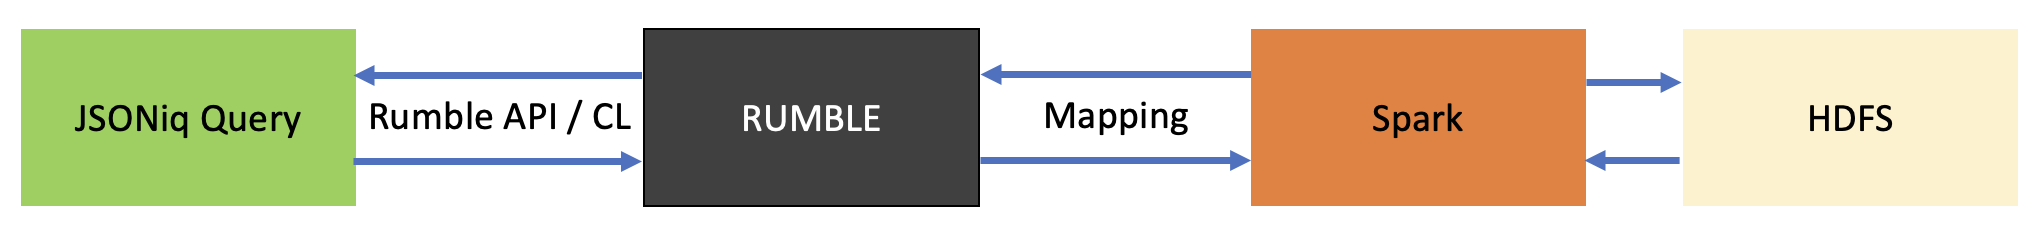
\includegraphics[width=\linewidth]{rumble_architecture.png}
	\caption{Rumble Architecture Overview}
	\label{fig:Rumble_Architecture}
\end{figure}

\subsection{Mapping}
\label{sec:RumbleMapping}
We said that Rumble has a logic that is capable of mapping the query to Spark primitives. We also said that in JSONiq, everything is a Sequence of Items. Therefore, Rumble uses interface Item in the code \cite{RumbleRepository}. All 6 types mentioned in Section \ref{sec:JSON} implement this interface. After that, the Item is wrapped using the Spark JavaRDD generic class or DataFrame if the Sequence of Items is structured and the mapping is complete. Spark is now able to execute queries using objects of the wrapper class.

As also said, FLWOR Expressions are the most powerful ones and we can view them as a set of clauses. Between themselves, clauses operate by consuming tuple streams instead of operating on Sequence of Items. Sequence of Items is produced only in the end with the mandatory Return clause. Therefore, in the code \cite{RumbleRepository}, Rumble uses class FlworTuple for wrapping to the Spark Dataset generic class that is used for DataFrames. For each clause, we have a RuntimeTupleIterator and they all, with the exception of Return, have a reference to FlworTuple. More details in Subsection \ref{sec:Generator}.

\subsection{General Architecture}
\label{sec:RumbleArchitecture}
So far, we were referring to Rumble as an engine. Essentially it is a compiler implemented in Java, and as such, it follows basic Compiler Design principles. In order not to break the declarative property of JSONiq query language, it requires proper separation of concerns. Irimescu in his thesis \cite{RumbleThesis} proposed the layered architecture described in Figure \ref{fig:Rumble_General_Architecture}. It consists of 4 main phases:
\begin{enumerate}
	\item Lexer and Parser take JSONiq query as an input and produce Abstract Syntax Tree - AST as the output 
	\item Translator takes the AST as the input and produces a tree of expressions - Expression Tree as the output
	\item Generator takes Expression Tree as input and converts it into a tree of runtime iterators - Runtime Iterator Tree
	\item Runtime iterators represent the code that can be executed on a single node or on top of Spark
\end{enumerate} 

\begin{figure}[h!]
	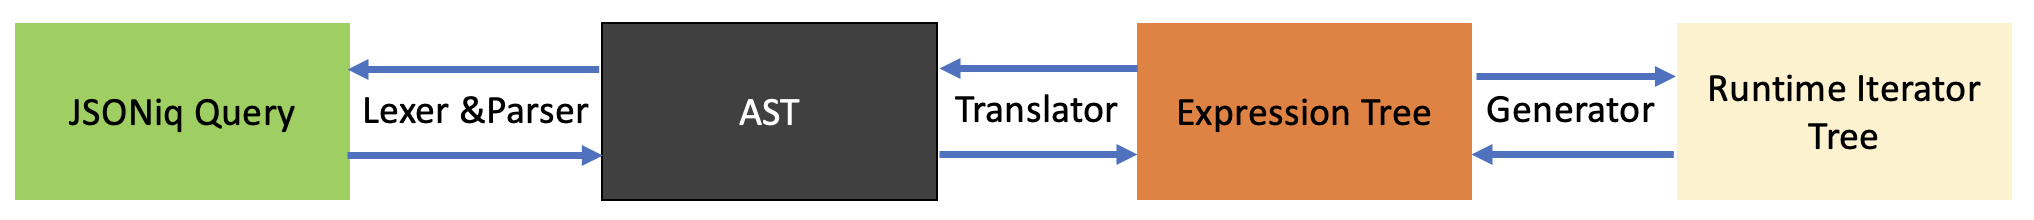
\includegraphics[width=\linewidth]{parsing_architecture.png}
	\vspace*{-5mm}
	\caption{Rumble General Architecture}
	\label{fig:Rumble_General_Architecture}
\end{figure}

\subsubsection{Lexer and Parser}
\label{sec:RumbleLexerParser}
The first steps in analyzing source code, in this case query written in JSONiq query language, are Lexical and Syntax analysis's performed by Lexer and Parser modules respectively. For rather simple languages, such as JSONiq, these two modules can be automatically generated from language grammar. Thus, Another Tool for Language Recognition - ANTLR v4 framework \cite{ANTLR} is used. ANTLR needs a grammar (.g4) file with definitions of all language constructs as the input. For Rumble, JSONiq.g4 file was implemented and using it ANTLR auto-generated Parser and Lexer together with BaseVisitor (implements visitor pattern) Java classes. In the code, we can first use the Lexer class that takes JSONiq query stream as input and then pass it to Parser class which will generate AST and conclude the so-called "front-end" part of the compiler.

\subsubsection{Translator}
In general with compilers, AST cannot be used directly. As explained in \cite{RumbleMLThesis}, JSONiq is a functional language that is composed of expressions. Thus, higher-level abstractions - Expression Tree is needed. To achieve higher-level abstractions, the following classes had to be implemented. On top of the inheritance tree, we have abstract class Node from which Expression and Clause classes are derived. Clause class is then used for deriving all clauses of FLWOR Expression. For all other Expression types mentioned in Section \ref{sec:JSONiq}, classes were derived from the Expression class. 

The second part of generating the Expression Tree required specific implementation of BaseVisitor class generated by ANTLR. BaseVisitor is a generic class and its specific implementation - TranslationVisitor class wraps around Node class. 

The third part of generating the Expression Tree is the Static Context class containing a map between variable names and sequence types. Each Expression has its own Static Context.

Using all these classes, it is then possible to generate th Expression Tree as explained in \cite{RumbleThesis}: 

"The visitor starts at the top-level Expression and then moves through all of the children passing along the current Static Context while doing three things:
\begin{enumerate}
	\item For any expression that it visits, it sets the Static Context to be equal to the currently generated one.
	\item For any variable reference, it checks that the variable name is present in the current Static Context, otherwise it throws an error (at compile time).
	\item For any variable declaration it creates a new Static Context containing the new variable and sets the previously existing Static Context as parent.
\end{enumerate}

\subsubsection{Generator}
\label{sec:Generator}
So-called "back-end" - the last part of the compiler includes code generation where the intermediate code gets transformed into assembly instruction and finally machine instructions. For this step in Rumble, we are performing conversion from Expression Tree to a tree of runtime iterators. As Rumble was written in Java, runtime iterators are in charge of executing operations that get converted to Java bytecode.

All RuntimeTupleIterator implement RuntimeTupleIteratorInterface while all other runtime iterators implement RuntimeIteratorInterface. Both interfaces are similar to java.util.Iterator interface with methods such as hasNext() and next(). Using next(), runtime iterators can iterate over Sequence of Items and return results one Item at a time. In addition, next() method triggers the computation of all children iterators by recursively calling next() method in them. Result of such implementation is "lazy evaluation", where results are computed only when demanded. 

These two runtime interfaces operate on Dynamic Context containing a map between variable names and actual sequences of items. Static Context is in charge of static type checking performed at compile-time, while Dynamic Context is in charge of dynamic type checking performed at runtime.

As pointed out in \cite{RumblePaper} "The main novelty in the design of Rumble is the runtime iterators that can switch dynamically between different execution modes, and which encode the decision of which nesting level is distributed." In total, there are 3 different execution modes. In local execution mode runtime iterators are executed on a single node locally in Java and they do not push computation to Spark. The other two, RDD-based execution (which uses Spark’s RDD interface) and  DataFrame-based execution (which uses the DataFrame interface), are executed on top of Spark. They both push computation to spark when a dataset is large and there is a clear advantage over local execution mode. The modes that a runtime iterator supports are based on JSONiq Expression category and presented in Table \ref{tab:RuntimeCategoriesMapping}. The column "As in JSONiq" represents classification as we have seen it before in Section \ref{sec:JSONiq} where Built-in Function and Sequence Construction are omitted since they are spread across several categories. The columns L, R and D represent local, RDD-based and DataFrame-based execution modes, respectively, while + signifies that this mode is supported.

\begin{table}[h!]
		\vspace{-1mm}
	\centering
	\resizebox{\textwidth}{!}{%
	\begin{tabular}{|l|l|l|l|l|l|} 
		\hline
		\textbf{Category}                      & \textbf{Expression/Clause}                                  & \textbf{As in JSONiq~}                                                                                                   & \textbf{L}         & \textbf{R}         & \textbf{D}          \\ 
		\hline
		\multirow{5}{*}{local-only}            & (),~\{\$k:\$v\},~[\$seq],~\$\$,~+,~-,~mod,~                 & \multirow{5}{*}{\begin{tabular}[c]{@{}l@{}}Arithmetic,\\Comparison,\\Logic,\\Literal,\\JSON construction\end{tabular}} & \multirow{5}{*}{+} & \multirow{5}{*}{}  & \multirow{5}{*}{}   \\ 
		\cline{2-2}
		& div,~idiv,~eq,~ne,~gt,~lt,~ge,~le,~and,~                    &                                                                                                                        &                    &                    &                     \\ 
		\cline{2-2}
		& or,~not,~\$a\textbar{}\textbar{}\$b,~\$f(\$x),~\$m~to~\$n,~ &                                                                                                                        &                    &                    &                     \\ 
		\cline{2-2}
		& try catch, instance~of, castable,                           &                                                                                                                        &                    &                    &                     \\ 
		\cline{2-2}
		& cast, some~\$x~in~\$y~satisfies...                          &                                                                                                                        &                    &                    &                     \\ 
		\hline
		\multirow{2}{*}{sequence-transforming} & \$seq[...],~\$a[\$i],~\$a[],~\$a[[]],~\$o.\$s,              & \multirow{2}{*}{JSON navigation}                                                                                       & \multirow{2}{*}{+} & \multirow{2}{*}{+} & \multirow{2}{*}{+}  \\ 
		\cline{2-2}
		& \$seq!..., annotate, treat                                  &                                                                                                                        &                    &                    &                     \\ 
		\hline
		\multirow{3}{*}{sequence-producing}    & json-file, parquet-file, libsvm-file,~                      & \multirow{3}{*}{}                                                                                                      & \multirow{3}{*}{+}  & \multirow{3}{*}{+} & \multirow{3}{*}{+}  \\ 
		\cline{2-2}
		& text-file, csv-file,~avro-file, root- file,                 &                                                                                                                        &                    &                    &                     \\ 
		\cline{2-2}
		& structured-json-file, parallelize                           &                                                                                                                        &                    &                    &                     \\ 
		\hline
		\multirow{3}{*}{sequence-combining}    & seq1,\$seq2, if (\$c) then... else...,                      & \multirow{3}{*}{}                                                                                                      & \multirow{3}{*}{+} & \multirow{3}{*}{+} & \multirow{3}{*}{+}  \\ 
		\cline{2-2}
		& switch (\$x) case... default...,                            &                                                                                                                        &                    &                    &                     \\ 
		\cline{2-2}
		& typeswitch (\$x) case... default...                         &                                                                                                                        &                    &                    &                     \\ 
		\hline
		\multirow{2}{*}{FLWOR}                 & for,~let,~where,~group~by,~                                 & \multirow{2}{*}{FLWOR}                                                                                                 & \multirow{2}{*}{+} & \multirow{2}{*}{}  & \multirow{2}{*}{+}  \\ 
		\cline{2-2}
		& order~by,~count, return                                     &                                                                                                                        &                    &                    &                     \\
		\hline
	\end{tabular}}
	\caption{Runtime iterator categorization for JSONiq expressions and clauses}
	\label{tab:RuntimeCategoriesMapping}
	\vspace{-3mm}
\end{table}

Local-only iterators executed in the local execution mode come down to implementing the Expression's behavior in Java. On the other hand, RDD and DataFrame-based execution modes require a mapping to Spark primitives as explained in Section \ref{sec:RumbleMapping}. There is an essential difference between these two modes that are running on top of Spark. The DataFrame-based mode is used in the case that internal structure is known statically. This mode is also preferred over RDD-based mode as it faster in execution. On the other hand, the RDD-based mode is used whenever the structure is unknown. 

Rumble, in its initial version, was using RDD-based mode for FLWOR Expressions. However, all FLWOR Clauses Iterators, with the exception of Return, operate with FlworTuple. From the query, it is possible to derive the static type of the variables in the tuples and therefore represent them as columns in DataFrame. Today, the RuntimeTupleIterator is using SQL queries instead of RDD transformations of Spark. We will not explain the mappings for each and every FLWOR Clause in detail, but we will make a parallel to For Clause and reuse an example from \cite{RumblePaper}. If the current variables are x, y, and z, and the new variable introduced by the for clause is i, then the for clause is mapped to the following:

SELECT x, y, z, EXPLODE(UDF(x, y, z)) AS i FROM input\_stream

Spark’s EXPLODE functionality corresponds to flatMap() on RDDs, while UDF is a Spark SQL user-defined function that takes all existing variables as input, and returns the resulting sequence of items as a List$<$Item$>$.

%Regarding all sequence category of runtime iterators, they all operate on sequences of items. Since item is essentially an interface and we have a polymorphic class hierarchy as all 6 JSON types implement it, we cannot use Dataframes but we use RDDs instead. Therefore, Sequence-transforming Expressions are handled using map(), flatMap(), and filter() transformations in Spark. Sequence-combining Expressions use RDD.union. There is a small exception for Sequence-producing Expressions. Only for json-file() and text-file() the structure is unknown, for all other file formats, structure is known and therefore Dataframe can be used. 